\chapter{Existierende Bibliotheken}
\label{cha:existirende_bibliotheken}

Bestehende Bibliotheken bieten eigene Visualisierungen von Regressionsmodellen an. In diesem Kapitel werden einige davon analysiert und mit den Anforderungen der Ziel-setzungen \ref{sec:Zielsetzung} und den Funktionen der Diagramme in Kapitel \ref{cha:Metriken_Diagramme} verglichen. Das Ziel ist es herauszufinden, welche Visualisierungen und Funktionalitäten bereits von bestehenden Bibliotheken abgedeckt werden.

\section{SlickML}
\label{sec:SlickML}
SlickML \parencite{slickml2020} ist eine Python-Bibliothek zur Entwicklung von Machinelearning-Modellen. Als Ziel setzt sich die Bibliothek "eine schnelle Experimentierung mit Modellen und maximale Ableitung von Informationen". Die Bibliothek\linebreak befindet sich noch in Entwicklung, bietet jedoch einzelne Funktionen zum Trainieren von Modellen, Hyperparameter-Optimierung sowie Sammlung und Visualisierung von Metriken.\\\\
\noindent Für Regressionsmodelle gibt es eine Funktion, welche Metriken aus Zielwerten sowie Vorhersage sammelt und visualisiert. Die generierten Diagramme und gewählten Metriken können dabei nicht beeinflusst werden. Bei den dargestellten Metriken handelt es sich um die Vorhersage relativ zu den Zielwerten, die Frequenz einzelner Vorhersagen, verschiedene Auswertungen vom Residuum, sowie der REC-Kurve (Abschnitt \ref{sec:roc_rec}).

%https://github.com/slickml/slick-ml
%https://docs.slickml.com/pages/quick_start.html
%https://www.docs.slickml.com/autoapi/slickml/metrics/index.html#slickml.metrics.RegressionMetrics

\section{Seaborn}
\label{sec:seaborn}

Seaborn \parencite{seaborn} ist eine Python-Bibliothek für Datenvisualisierung, welche auf Matplot aufbaut. Die Bibliothek stellt die API von Matplot auf einer höheren Ebene zur Verfügung. Anwender:innen wird dadurch ermöglicht, einfach attraktive Visualisierungen von Datensätzen zu erstellen.\\\\
\noindent Die Bibliothek unterstützt eine Vielzahl an implementierten Diagrammen. Diese können mithilfe eines einzelnen Aufrufs zur Visualisierung von Datensätzen verwendet werden. Jedes dieser Diagramme kann mithilfe von visuellen Themen und einem eigenen Objekt-Interface weiter angepasst werden. Außerdem ist es möglich, mehrere Diagramme zu einer gemeinsamen, komplexeren Visualisierung zusammenzufügen. Ein Beispiel dafür ist in Abbildung \ref{fig:example_seaborn} zu sehen. Seaborn besitzt jedoch keine explizite Unterstützung für interaktive Diagramme.

\begin{figure}[H]
    \centering
    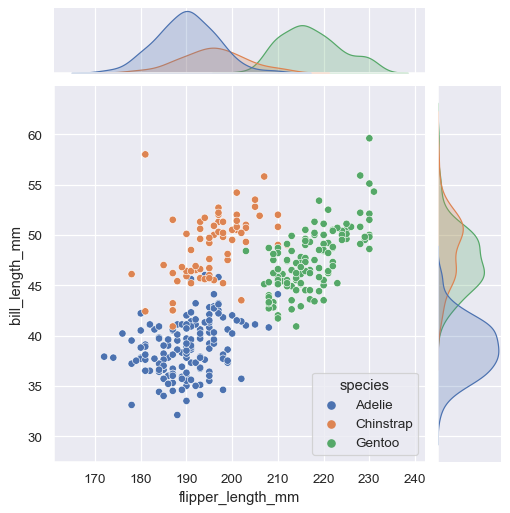
\includegraphics[height=.6\textwidth]{images/seaborn_example.png}
    \caption{Beispiel eines Streudiagramms mit Randverteilung in Seaborn\protect\footnotemark}
    \label{fig:example_seaborn}
\end{figure}

\footnotetext{Quelle: https://seaborn.pydata.org/tutorial/introduction.html}

% https://joss.theoj.org/papers/10.21105/joss.03021
% https://seaborn.pydata.org/
% https://seaborn.pydata.org/tutorial/function_overview.html#similar-functions-for-similar-tasks
% https://seaborn.pydata.org/tutorial/regression.html?highlight=regression
% https://seaborn.pydata.org/examples/index.html


\section{Plotly}
\label{sec:plotly}

Plotly\footnote{https://github.com/plotly/plotly.py} ist eine Bibliothek für interaktive Visualisierung, mit Unterstützung von Python. Sie besitzt ebenfalls Implementierungen für R, Julia, Javascript, sowie andere Sprachen. Die Bibliothek ermöglicht verschieden 2D- und 3D-Diagramme, sowie Visualisierungen für Karten.\\\\
\noindent Alle Diagramme besitzen automatisch eine Zoom-Funktion, Tooltips sowie die\linebreak Möglichkeit den Bildbereich zu verschieben. Die Visualisierungen können sowohl\linebreak Lokal, im Web und auch in Jupyter-Notebook dargestellt werden. Neben einer Vielzahl\linebreak anderer Diagramme werden auch Liniendiagramm, Streudiagramm und Blasendiagramm\linebreak unterstützt. Die zusätzliche Interaktivität beschränkt sich hier jedoch auf das Ein- und Ausblenden von Datenklassen. Zusätzliche Funktionen wie eine dynamische Wahl der Metriken können jedoch eigenständig implementiert werden. Dafür bietet die\linebreak Bibliothek Unterstützung für UI-Elemente wie Knöpfe und Drop-Down-Elemente.\linebreak Dementsprechend konkurriert diese Bibliothek hauptsächlich mit Matplot.

\begin{figure}[H]
    \centering
    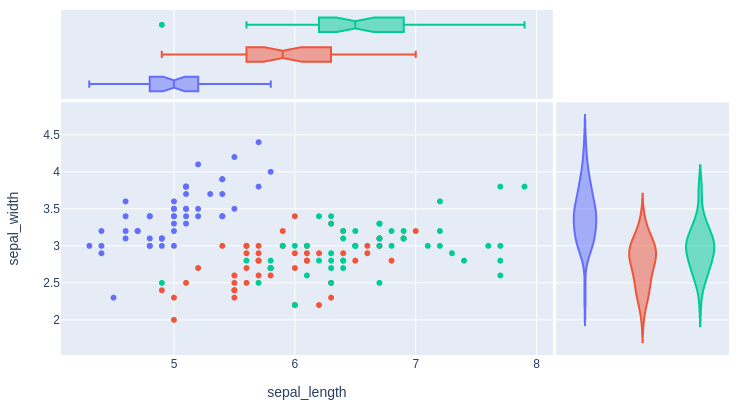
\includegraphics[height=.6\textwidth]{images/plotly_example.png}
    \caption{Beispiel eines Streudiagramms mit Randverteilung in plotly\protect\footnotemark}
    \label{fig:example_plotly}
\end{figure}

\footnotetext{Quelle: https://plotly.com/python/marginal-plots/}

% https://github.com/plotly/plotly.py
% https://plotly.com/python/
% https://plotly.com/python/ml-regression/

\section{Ergebnis}

Es gibt aktuell eine gute Auswahl an Bibliotheken welche, sich mit dem Thema Visualisierung beschäftigen. Wie in der Problemstellung angemerkt, schafft es jedoch keine den Anforderungen von Scikit-charts genau zu entsprechen.\\
\begin{itemize}
    \item Die Visualisierung in SlickML ist statisch und zu spezifisch. 
    \item Seaborn bietet eine gute Erweiterung von Matplot an. Die Bibliothek ist außerdem einfach zu verwenden. Sie bietet jedoch keine erweiterte Unterstützung von dynamischen Interaktionen.
    \item Plotly bietet dynamische Visualisierungen und eine gute Integration in Jupyter Notebooks, sowie Webseiten. Der Umfang der Funktionen entspricht jedoch nicht dem Umfang, welcher in dem Kapitel \ref{cha:Metriken_Diagramme} identifiziert wurden.
\end{itemize}

\vspace{\baselineskip}

\noindent Alle diese Bibliotheken besitzen dementsprechend Einschränkungen bezüglich der\linebreak Aufgabenstellung. Trotzdem bieten Sie eine gute Basis um Visualisierungen in ein\linebreak Projekt einzubauen. Die Bibliothek dienen außerdem als eine Inspiration für die\linebreak Implementierung von Scikit-charts.

% Referenz auf Problemstellung -> Zu einfach und Statisch, erneut aufwand notwendig, inflexibel. Keine komplette Abdeckung der Zielsetzung jedoch